\chapter{Introduction}\label{Ch1}

\section{General Information}

This project proposal is presented as one of the partial requirements to aspire to the degree of Bachelor of Science in Mechanical Engineering, and is possible through the "KOSPIE" scholarship program, a collaborative effort between the Universidad del Valle and the German Academic Exchange Service (DAAD). In partnership with Procter \& Gamble Manufacturing GmbH.

For this case, the project will be run under the Femcare Ultra Pads Section in the Operations and Manufacturing Department located in Crailsheim, Germany. It will be part of the currently existing research and development projects in the field of Scrap Reduction and Optimization. 

\textbf{Important to notice:} All documents regarding this project contain confidential information of 
Procter \& Gamble Manufacturing GmbH, which is subject to secrecy. These papers are therefore only to be made 
accessible to the responsible members of the Academic Program of Mechanical Engineering and 
the members of the examination board of the Universidad del Valle. The disclosure and publication 
of the content as a whole or in part to third parties is prohibited. It is not permitted to make 
transcripts or copies in any form. Exceptions require the written approval of Procter \& Gamble Manufacturing GmbH. All rights to 
acquire and register industrial property rights, in particular to register patents, utility models and/or 
designs, are also reserved by the company Procter \& Gamble Manufacturing GmbH. 

This blocking notice is valid until May 5th, 2029.

\section{Justification}
%
A sanitary Ultra Pad is composed by a 4 main materials and has a layered structure,in which the most critical layers are the Second-Top-Sheet (STS) and the Core, not only because of their Properties, but because of their overall performance. The Top-Sheet (TS) is the material layer that goes in direct contact with the skin, the Second-Top-Sheet (STS) is an intermediate layer that connects the TS and the absorbent layer, the core (C); the Back-Sheet (BS) is the final layer and its the one in contact with the underwear. A single pad is stored in a bag called Pouch, when it has wings, these are folded and glued using an One-Piece-Tape (OPT); each Pouch is folded and sealed using a Reseal-Tape (RST).  All this materials are attached to one another using different glues such as: the Anti-Wrinkle-Adhesive (AWA), the Core-Integrity-Adhesive (CIA),  the Wing-Laminated-Adhesive (WLA), the Panty-Fastening-Adhesive (PFA), and the Shield-Fastening-Adhesive.  See Figure~\ref{Layer}. 
%
\begin{figure}[H]
    \centering
    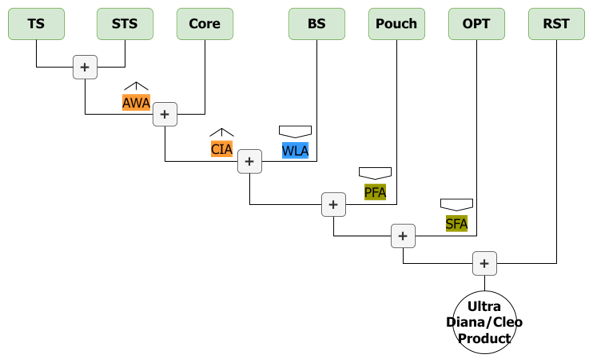
\includegraphics[scale=0.5]{FIGURES/Layers.png}
    \caption{Ultra Pad Material Layers including Glues and Bag~[Author].}
    \label{Layer}
\end{figure}

In the Crailsheim Plant, there are seven Lines currently in operation producing Ultra Pads, the lines are working (almost) at a constant rhythm and only stopping when necessary: for Unplanned-Downtime (when a Module Fails or if an unexpected error arises), for Planned-Downtime (cleaning, format change, etc.), for Filter Cleaning (a weekly overall Plant stop for cleaning  and performing checking activities in the main air system). These Lines run at an average speed of $1220$ Pads-per-Minute (PPM), the speed depends mostly on the PO (Purchase Order) and the PR (Production Rate), which is the production requirement and determines the number of Wickets that are going to be produced in one shift. The STS-Foldover Error accounts (in the worst case scenario) for near the $30\%$ of the whole production ($3\%$ of the global percentage).

The frequent occurrence of a rejection labelled as \textit{"Foldback"} is at the moment a significant challenge that leads leading to substantial scrap and waste, mainly in the STS Material Layer. This issue occurs on the STS Cut-and-Lay (STS C\&L) Module of the Lines, and not only hinders production efficiency but also results in increased operational costs and a heightened environmental footprint. While quality control measures are in place, the persistence of Foldbacks underscores the need for a thorough analysis of their root causes and the development of targeted interventions. Through this manufacturing process, various materials (including special glues and coatings) interact with one another. 
%%
\section{Problem Statement}
%
Although tracking of operating conditions across different lines is facilitated by the implementation of a range of sensors and data acquisition systems, yet the root cause of Foldbacks remains unclear, as it exhibits limited correlation with various parameters. Despite this, certain parameters such as Line Speeds, Material Properties, Web Path, etc. are not to be modified. Hence, the following question arises: What innovative methodology and process improvement can be employed to reduce the occurrence of Foldback rejections without modifying the Base Condition of the Lines?
%%
\section{Objectives}

\textbf{General Objective}

Propose an effective strategy for scrap reduction due to foldbacks in the manufacturing process of sanitary Pads.

\textbf{Specific Objectives}

\begin{itemize}
    \item[\textbf{--}]  Identify the improvement areas in the STS C\&L Module on the current pad manufacturing process.
    \item[\textbf{--}]  Propose improvements on the STS C\&L Module for mitigation of foldbacks occurrence.
    \item[\textbf{--}] Evaluate the impact of the given proposal on the overall production efficiency. %and waste generation. 
    %\item[\textbf{--}]  Design process improvements to mitigate the occurrence of foldbacks.
    %\item[\textbf{--}]  Implement the designed process improvements and monitor their impact. 
\end{itemize}
%%
\section{Theoretical Framework and State of the Art}
%%
The Web Foldover or Foldback, also known as wrinkling, and Web buckling are intricate phenomena that occur in continuous manufacturing processes, particularly in industries such as paper production, textiles, and thin film manufacturing, see Figures~\ref{foldback} and~\ref{defect1}. These phenomena arise as a result of the complex interactions between the web material and processing equipment, leading to undesirable quality defects and increased scrap rates~\cite{Hashimoto2007PredictionMO,rosiumconference}. 

The measurement of web stresses during roll winding is a crucial aspect of understanding and mitigating these issues. Existing methods for measuring roll structure variables, such as stress and strain, have been found to be unreliable, necessitating the development of new measurement techniques. Researchers have made efforts to improve the hardware and software used for density measurement and have reviewed winding models to establish connections between stress models and experimental measurements. In the paper industry, the components of a winder play a significant role in the winding process. For instance, the unwind stand securely holds the parent roll and allows for straight buildup of the roll edges, while the guide roller helps maintaining web geometry and tension evenness. Spreader rollers are employed to lay the web flat and spread individually cut webs, and the windup section includes rollers or drums to enhance web tension and eliminate entrained air. Fully automated winders also incorporate equipment for core insertion, web fastening to cores, and finished roll ejection. Sensors, actuators, and controllers are employed to ensure effective control of the winding process~\cite{rosiumconference,roisum1990measurement}. 
\begin{figure}[H]
        \centering
    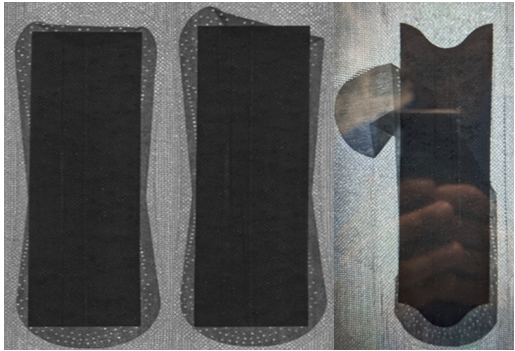
\includegraphics[width=0.55\linewidth]{FIGURES/foldback.png}
    \caption{Foldback Rejection from Vision System in one of the Lines~[Author].}
    \label{foldback}
\end{figure}

\begin{figure}[H]
    \centering
    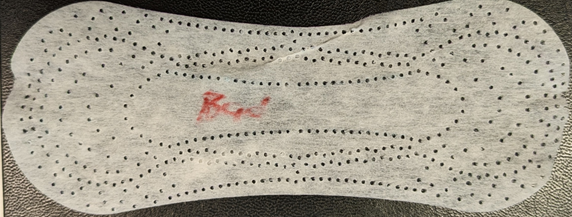
\includegraphics[width=0.6\linewidth]{FIGURES/defect1.png}
    \caption{STS Material Layer with Foldback Defect~[Author].}
    \label{defect1}
\end{figure}

The winding processes are influenced by two primary factors: productivity and quality. Productivity refers to the ability of the winder and its operators to match or surpass the output of preceding processes. Falling behind in winding can lead to a decrease in overall output. On the other hand, Material-Roll quality is of paramount importance, as rolls failing to meet customer requirements must either be salvaged or scrapped. Roll quality defects can arise either prior to winding or during the winding process itself, with issues such as tears, starring, and telescoping being common examples. 

\begin{figure}[H]
    \centering
    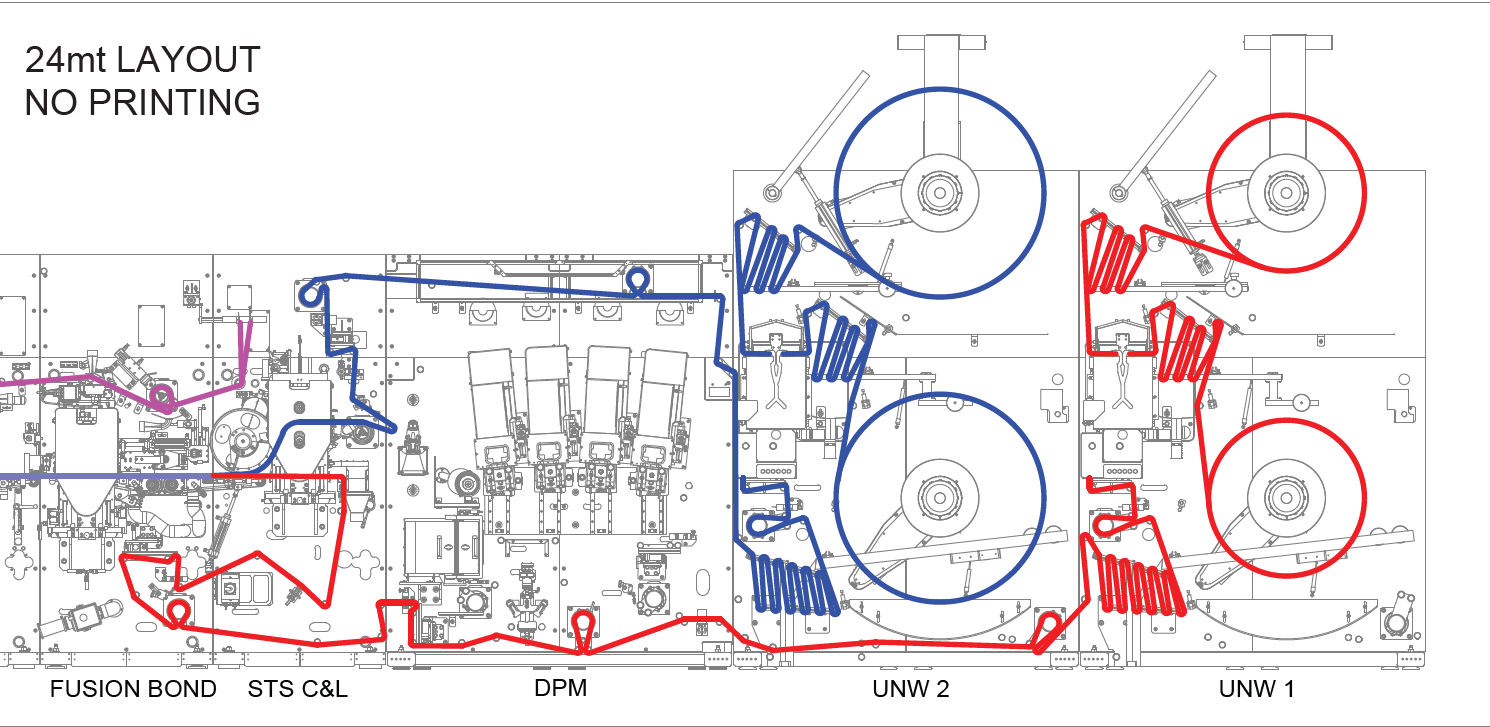
\includegraphics[scale = 0.3]{FIGURES/layout.png}
    \caption{Web Path Layout from Unwind Module to fusion-Bond Module in one of the Lines at P\&G~\cite{layout}}
    \label{layout}
\end{figure}


To control the winding process, operators adjust key parameters known as the Torque, Tension, Speed, Vacuum Power, Material Length, etc. These parameters can be manipulated to regulate the winding process, affecting the production efficiency and the material itself. However, there are limits to the extent to which these parameters can be adjusted. The torque is constrained by friction, the tension should not be too low or too high, and the vacuum power is limited by the general air and plant ventilation system. The material properties also play a significant role in roll structure. Properties such as the caliper (thickness), web, density, yield and tensile strengths, and coefficient of friction can influence roll structure, but not all properties have a direct effect. Web properties are typically specified based on end-use requirements and are not directly modifiable outputs of the winding system~\cite{CriticalWebWrinklingLie2020}. Figure~\ref{layout} shows a schematic view of the Roll-Unwinding Modules (UNW), the Digital-Printer-Module (DPM), the STS C\&L, and the Fusion-Bond Module of one the lines of P\&G in Crailsheim, each colored line represents a different material web, and each change of path direction corresponds to the point in which a roll or and an actuator is placed.

In the field of winding modeling, researchers have developed mathematical models to describe the physics of wound rolls and predict roll structure. These models employ constitutive equations to characterize the behavior of the material and can be implemented in computer simulations for optimization purposes. However, modeling roll structure presents challenges, as early models based on simplified assumptions and equations had limited accuracy. As the understanding of wound roll behavior improved, more advanced models were developed, incorporating realistic assumptions and equations, such as non-linear material behavior and core stiffness considerations. Numerical methods, including Finite Element Analysis (FEA), were employed to solve the complex equations and simulate the behavior of wound rolls more accurately~\cite{Hashimoto2007PredictionMO,rosiumconference}. 

One crucial aspect of wound roll modeling is the determination of boundary conditions, as they play a pivotal role in solving the differential equations that describe the stress distribution within the roll. Boundary conditions include core stiffness and wound-in-tension at the outer surface of the roll. Core stiffness is influenced by core material and geometry, while wound-in-tension reflects the tension applied to the web during the winding process~\cite{walker2009taxonomy}. 

%Accurately modeling wound rolls  also requires considering the incremental nature of winding, where stresses are incrementally added with each wrap of material. To simulate this behavior effectively, stress profiles at each step must be calculated and added to the existing stresses. 

While wound roll and web modeling has evolved to provide more accurate predictions of web stresses within the roll, challenges remain in accurately capturing their complex behavior. Factors such as hygroscopic behavior, deflections, and geometry variations pose ongoing challenges, necessitating further research to enhance the accuracy and applicability of wound roll models.

Furthermore, the properties of materials pose a significant concern that impacts not only the occurrence of wrinkling or folding but also exerts substantial influence on the overall performance of the web during the entire manufacturing process. These properties play a pivotal role from the initial stages of material production to the final assembly of the product. As a result, meticulous attention is given to ensuring that all materials used in production adhere to the most stringent quality standards. Hence, any attempts to enhance or modify materials must be approached with utmost caution and precision.

As a consequence of this, a "Module Focused" approach is suggested by many authors, i.e., to find implementations and improvements for the Line Modules instead of going directly to modify the Materials. This approach offers more flexibility when it comes to Production terms, as the materials are always subjected to constant development, whereas the Modules do not. However, this approach corresponds to the modification of the Cutting, Fusion-Bonding, or Cut-and-Slip units, as well as the Conveyor Belt System that drives the Web, the Piping, and the Pneumatic System. 

Recent studies have highlighted the role of friction in the formation of wrinkles in web materials~\cite{Hashimoto2007PredictionMO}. The interaction between the web and the rollers can lead to undesirable surface defects and compromise the overall quality of the product. To mitigate this issue, the implementation of a thin air layer supported by a carefully calibrated vacuum system has shown promise. By effectively managing the flowrate and speed requirements, this approach aids in the proper handling of the web, reducing the occurrence of wrinkles. Moreover, it has been observed that this technique also contributes to effective dust and particle control~\cite{Xu2016}. The careful control of the vacuum system not only improves the handling of the web but also enhances the overall cleanliness and quality of the final product (Figure~\ref{roll1}). These findings underscore the significance of optimizing the vacuum system parameters to minimize friction-related defects and ensure superior web performance. 
%
\begin{figure}[H]
    \centering
    \includegraphics[width=0.5\linewidth]{FIGURES/Roll1.png}
    \caption{Schematic View of different anomalies in winding rolls~\cite{rosiumconference}}
    \label{roll1}
\end{figure}
%%

